\documentclass[../ZF_SWEN1.tex]{subfiles}

\begin{document}

\paragraph{Definition: } Vereinfachtes UML-Klassendiagramm.

\paragraph{Aufbau: } Fachliche Begriffe mit ihren Attributen, setzt Begriffe in Beziehung zueinander.\\
Geht nur um die Problemstellung und das Fachgebiet.


\subsection{Domänenmodell als vereinfachtes UML Klassendiagramm}

\textbf{Konzepte = }Klassen \\
\textbf{Eigenschaften = }Attributen (Typenangabe entfällt) \\
\textbf{Assoziatonen = }Beziehungen zwischen Konzepte mit Multiplizitäten an beiden Enden.\\
\paragraph{Nur wenn es einen guten Grund gibt:\\}
\begin{itemize}
	\item \textbf{Aggregation = }Keine echte Semantik, als Abkürzung für "hat".
	\item \textbf{Komposition = }z.B wenn Produktkatalog gelöscht wird, dann auch die darin enthaltenen Produktbeschreibungen. Abkürzung "bietet an".
\end{itemize}

\begin{multicols}{3}
\begin{figure}[H]
	\centering
	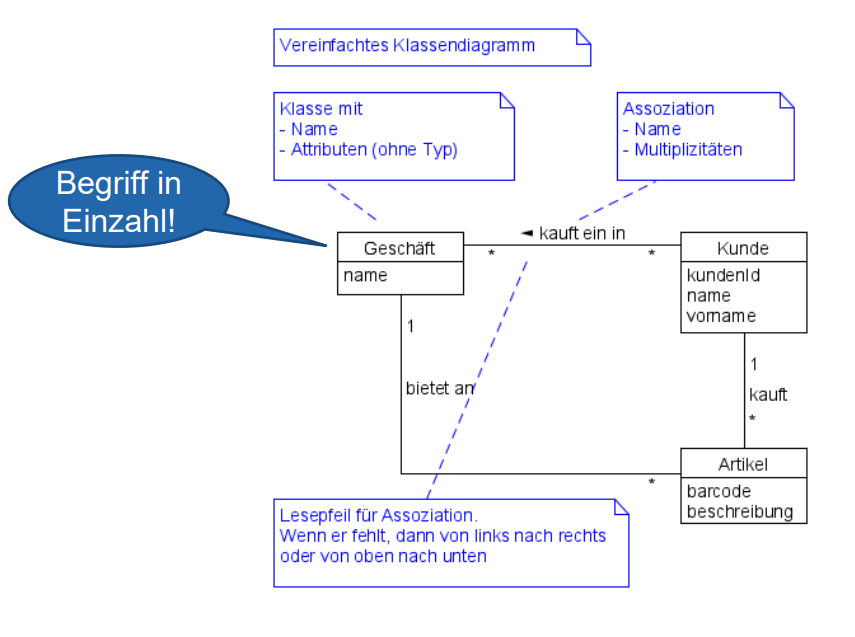
\includegraphics[width=0.3\textwidth] {Resources/Images/DM1.png}
	\caption{\label{fig:DM1}DM1}
	\end{figure}


\columnbreak
\begin{figure}[H]
	\centering
	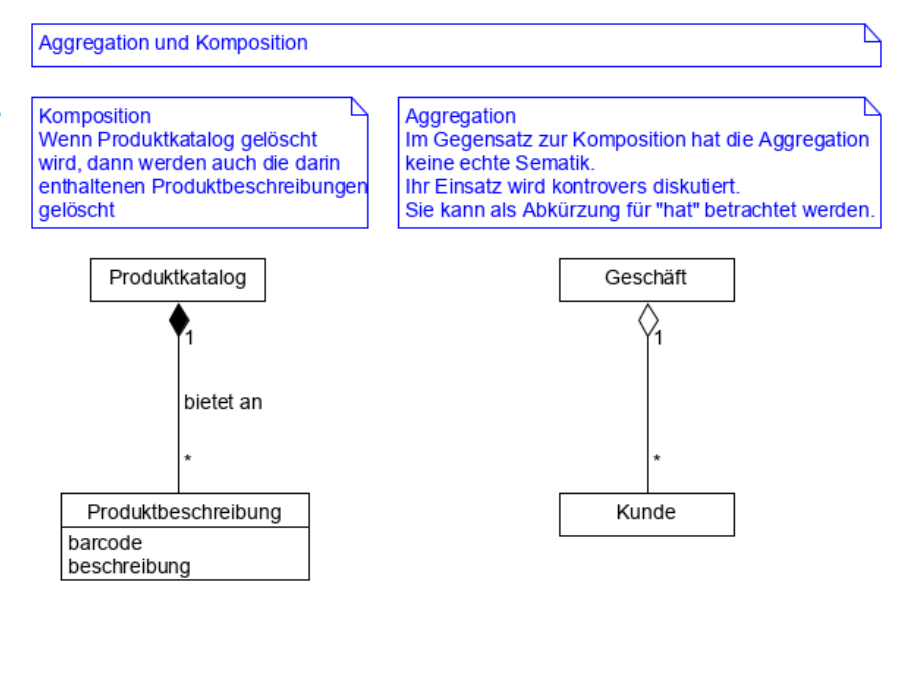
\includegraphics[width=0.3\textwidth] {Resources/Images/DM2.png}
	\caption{\label{fig:DM2}DM2}
	\end{figure}
\columnbreak
\begin{figure}[H]
	\centering
	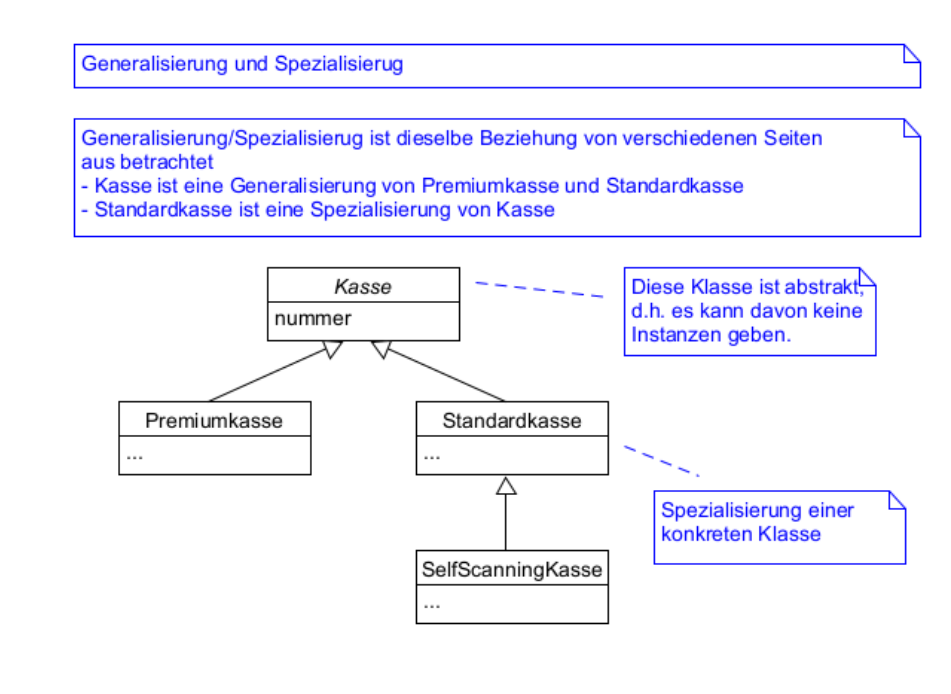
\includegraphics[width=0.3\textwidth] {Resources/Images/DM3.png}
	\caption{\label{fig:DM3}DM3}
	\end{figure}
\end{multicols}


\subsection{Vorgehen}

\begin{enumerate}
	\item Konzepte identifizieren
	\begin{enumerate}
		\item Fachwissen und Erfahrung verwenden
		\item Substantive aus Anwendungsfällen
		\item Kategorienliste verwenden
	\end{enumerate}
	\item Attributen
		\begin{enumerate}
		\item Fachwissen verwenden
	\end{enumerate}
	\item Konzepte in Verbindung zueinander setzen
			\begin{enumerate}
		\item Fachwissen verwenden
		\item Kategorienliste verwenden
	\end{enumerate}
	\item Auftraggeben und/oder Fachexperten beiziehen
	\item Vorgehensweise eines Kartografen
	
\end{enumerate}

\subsubsection{Kategorienliste}

\begin{multicols}{3}
\begin{figure}[H]
	\centering
	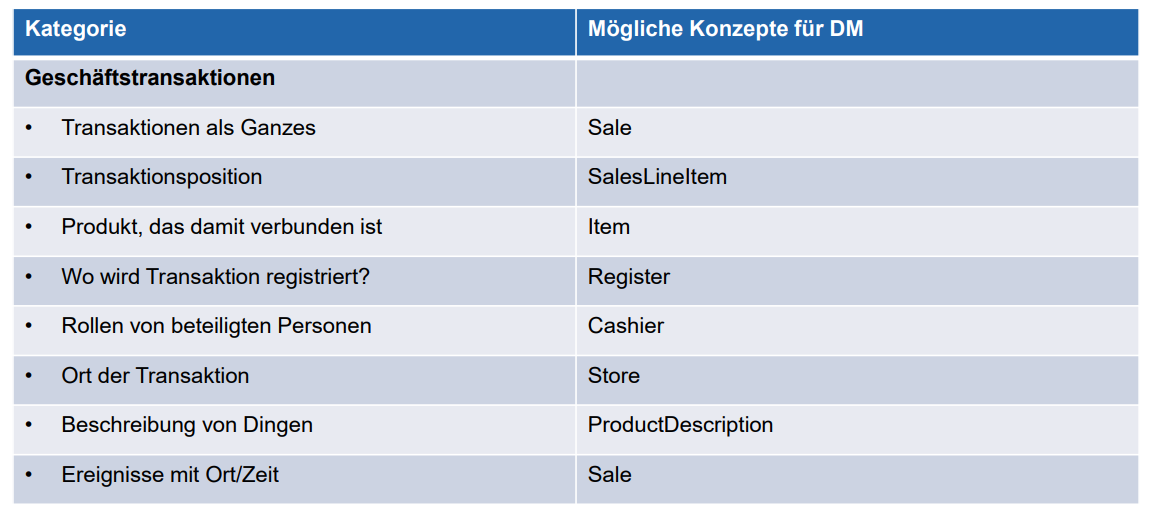
\includegraphics[width=0.3\textwidth] {Resources/Images/Kategorienliste1.png}
	\caption{\label{fig:Kategorienliste1}Kategorienliste1}
	\end{figure}


\columnbreak
\begin{figure}[H]
	\centering
	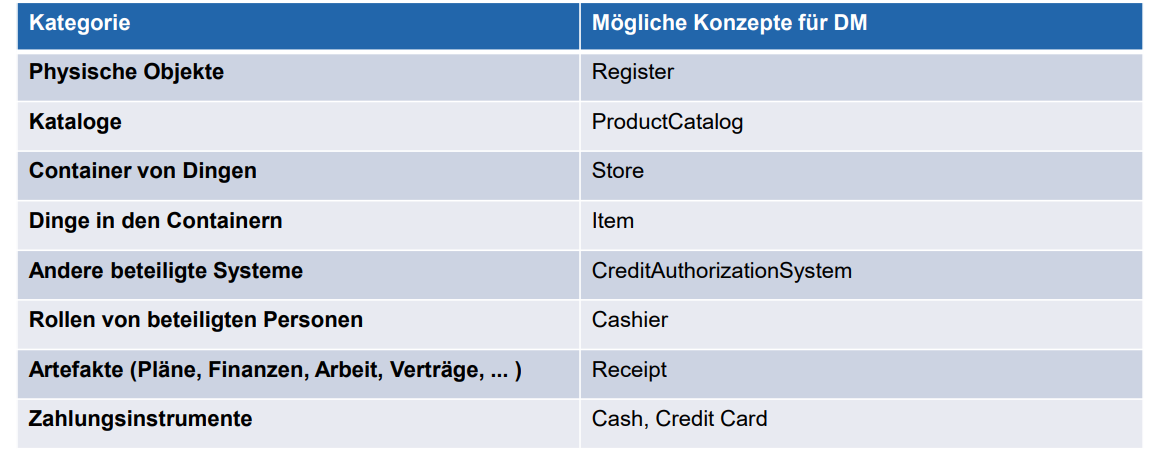
\includegraphics[width=0.3\textwidth] {Resources/Images/Kategorienliste2.png}
	\caption{\label{fig:Kategorienliste2}Kategorienliste2}
	\end{figure}
\columnbreak
\begin{figure}[H]
	\centering
	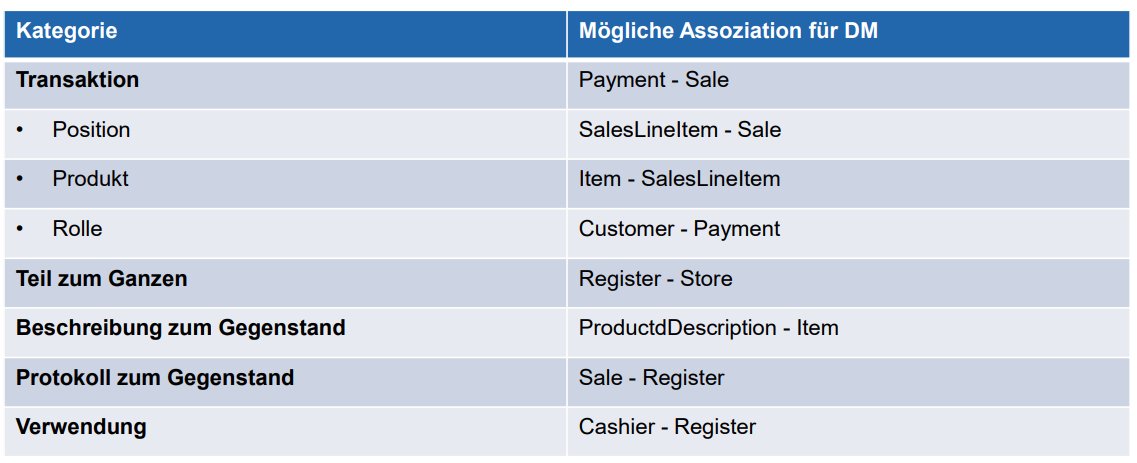
\includegraphics[width=0.3\textwidth] {Resources/Images/Kategorienliste3.png}
	\caption{\label{fig:Kategorienliste3}Kategorienliste3}
	\end{figure}
\end{multicols}

\subsection{Datentypen von Attributen}

\begin{itemize}
	\item Wenn nötig: eigene Datentypen als \textbf{Konzepte}
	\item Dann definieren wenn:
	\begin{itemize}
		\item Typ aus mehreren \textcolor {violet}{Abschnitten} (wie Tel.Nr)
		\item \textcolor {violet} {Operationen} darauf sind möglich (Validierung Kreditkartennummer)
		\item Hat selber \textcolor {violet}{eigene Attribute} (Verkaufspreis mit Anfangs \& Enddatum)
		\item \textcolor {violet}{Verknüpft} mit Einheit (Preis mit Währung)
	\end{itemize}
	
\end{itemize}


\subsubsection{Anti-Pattern}

\paragraph{Assoziationen statt Atrribute\\}
\begin{multicols}{2}
\begin{figure}[H]
	\centering
	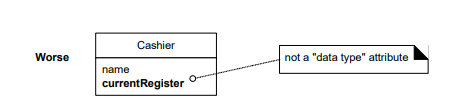
\includegraphics[width=0.3\textwidth] {Resources/Images/AntiPattern1.png}
	\caption{\label{fig:AntiPattern1}AntiPattern Bad}
	\end{figure}
\columnbreak
\begin{figure}[H]
	\centering
	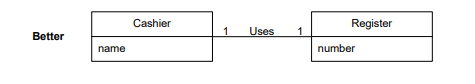
\includegraphics[width=0.3\textwidth] {Resources/Images/AntiPattern2.png}
	\caption{\label{fig:AntiPattern2}AntiPattern Good}
	\end{figure}
\end{multicols}

\subsection{Vorgehensweise eines Kartografen}

\begin{itemize}
	\item Vorhandene Begriffe oder Wissen einsetzen (Gebiete besuchen, Bewohner nach Begriffen befragen)
	\item Unwichtiges weglassen
	\item Nichts hinzufügen, was es (noch) nicht gibt 
	\begin{itemize}
		\item 	\textcolor {red} {Ausnahme:} System, das enwickelt wird, kann eingetragen werden
	\end{itemize}
	\item Nur analysieren, (noch) keine Lösungen entwerfen

\end{itemize}

\title {Keine Software Klassen im Domänenmodell :}

\begin{figure}[H]
	\centering
	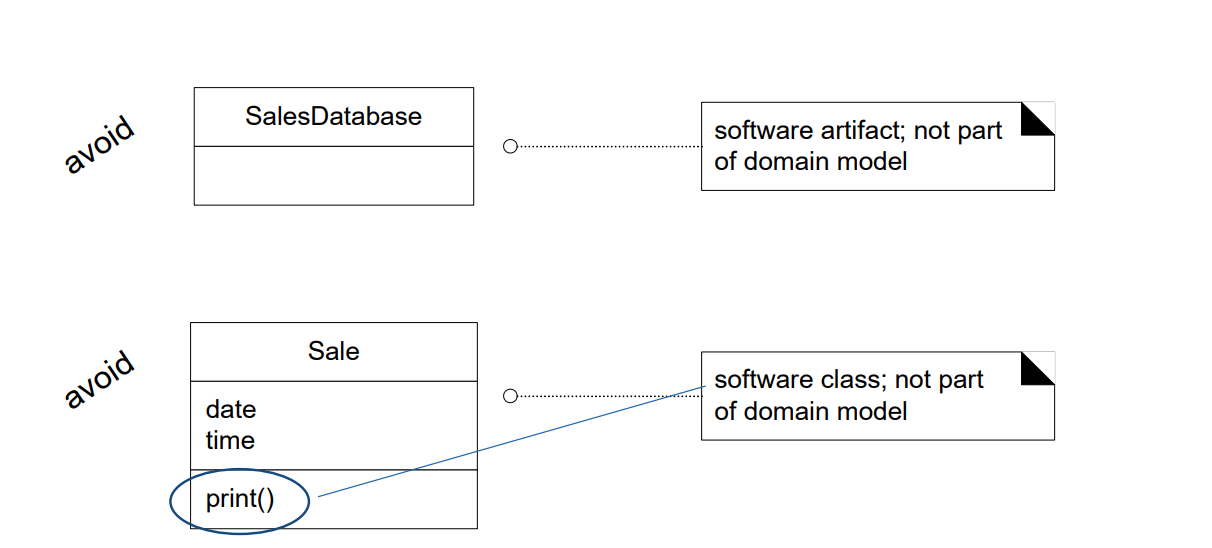
\includegraphics[width=0.3\textwidth] {Resources/Images/AntiPatternSoftware.png}
	\caption{\label{fig:AntiPatternSoftware}AntiPatternSoftware}
	\end{figure}


\subsection{Domänenmodell vollständig Beispiel}

\begin{figure}[H]
	\centering
	\includegraphics[width=0.3\textwidth] {Resources/Images/BeispielDomänenmodell.png}
	\caption{\label{fig:BeispielDomänenmodell}BeispielDomänenmodell}
	\end{figure}


\subsection{Analysemuster}
\begin{itemize}
	\item \textcolor {teal} {\textbf{Beschreibungsklassen}}
	\begin{itemize}
		\item Item = Physischer Gegenstand oder Dienstleistung
		\item Mehrere Artikel desselben Typs
		\item Attribute (description, price, serial number, itemID)
			\begin{multicols} {2} \begin{figure}[H]
				\centering
				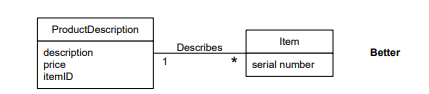
\includegraphics[width=0.3\textwidth] {Resources/Images/Beschreibungsklassen.png}
			\caption{\label{fig:Beschreibungsklassen}Beschreibungsklassen}
	\end{figure} 
	\columnbreak 
	\begin{figure}[H]
	\centering
	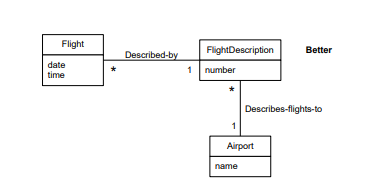
\includegraphics[width=0.3\textwidth] {Resources/Images/BeschreibungsklasseFlug.png}
	\caption{\label{fig:BeschreibungsklasseFlug}BeschreibungsklasseFlug}
	\end{figure} 
			\end{multicols}
	\end{itemize}
	\item \textcolor {teal} {\textbf{Generalisierung / Spezialisierung}}
	\begin{itemize}
		\item Spezialisierung als "is a" Beziehung zu 
					\begin{multicols} {2} \begin{figure}[H]
				\centering
				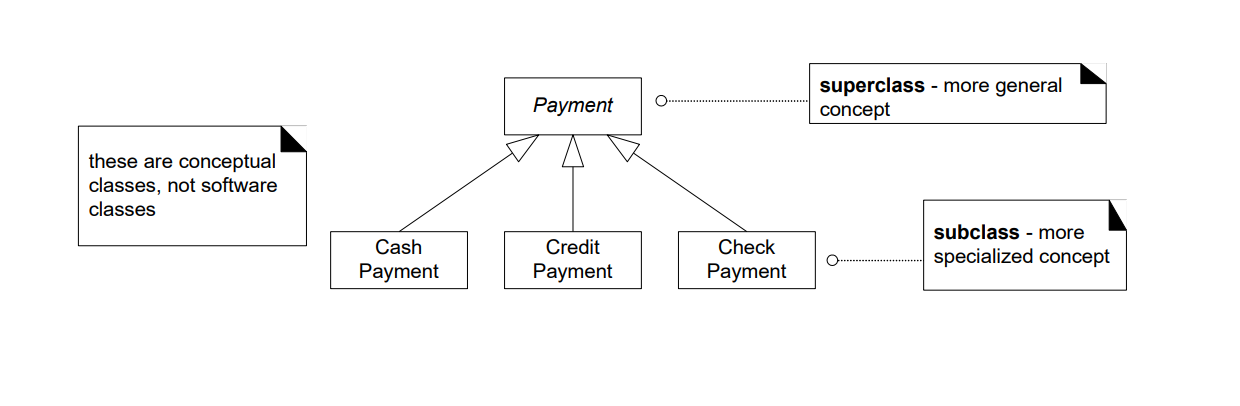
\includegraphics[width=0.3\textwidth] {Resources/Images/GeneralisierungSpezialisierung.png}
			\caption{\label{fig:GeneralisierungSpezialisierung}GeneralisierungSpezialisierung}
	\end{figure} 
	\columnbreak 
	\begin{figure}[H]
	\centering
	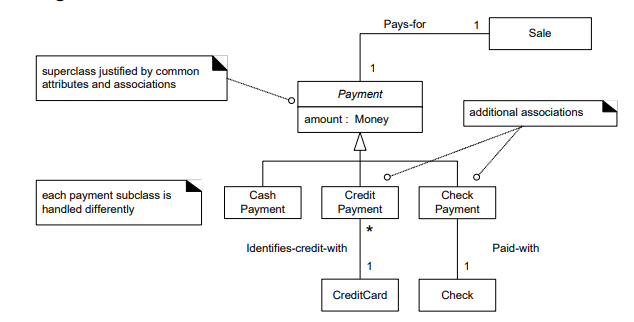
\includegraphics[width=0.3\textwidth] {Resources/Images/GeneralisierungSpezialisierungAttribute.png}
	\caption{\label{fig:GeneralisierungSpezialisierungAttribute}GeneralisierungSpezialisierungAttribute}
	\end{figure} 
			\end{multicols}
	\end{itemize}
	\item \textcolor {teal}{\textbf{Komposition}}
	\item \textcolor {teal} {\textbf{Zustände}}
		\begin{itemize}
		\item Eigene Hierarchie für Zustände definieren: \begin{figure}[H]
				\centering
				\includegraphics[width=0.3\textwidth] {Resources/Images/Zustände.png}
			\caption{\label{fig:Zustände}Zustände}
	\end{figure} 
	\end{itemize}
	\item \textcolor {teal} {\textbf{Rollen}}
	\begin{itemize}
		\item Dasselbe Konzept kann unterschiedliche Rollen einnehmen: \begin{multicols} {2} \begin{figure}[H]
				\centering
				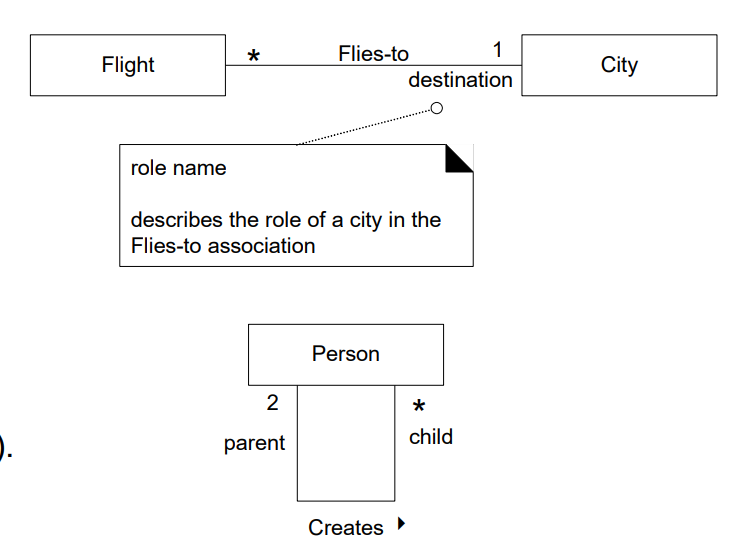
\includegraphics[width=0.3\textwidth] {Resources/Images/DMRolleName.png}
			\caption{\label{fig:DMRolleName}DMRolleName}
	\end{figure} 
	\columnbreak 
	\begin{figure}[H]
	\centering
	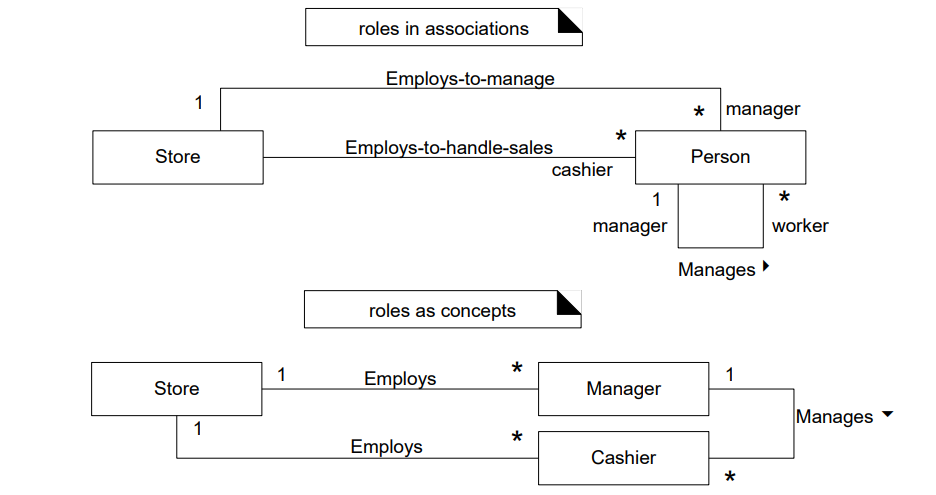
\includegraphics[width=0.3\textwidth] {Resources/Images/DMRolleKonzept.png}
	\caption{\label{fig:DMRolleKonzept}DMRolleKonzept}
	\end{figure} 
			\end{multicols}
	\end{itemize}
	\item \textcolor {teal} {\textbf{Assoziationsklasse}}
	\begin{itemize}
		\item Wenn Assoziationen eigene Attribute haben (MerchantID für Kreditkarte Geschäft<->AuthorizationService): \begin{figure}[H]
				\centering
				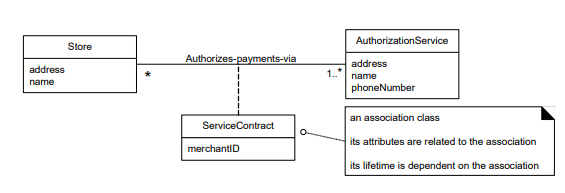
\includegraphics[width=0.3\textwidth] {Resources/Images/Assoziationsklasse.png}
			\caption{\label{fig:Assoziationsklasse}Assoziationsklasse}
	\end{figure} 
	\end{itemize}
	\item \textcolor {teal} {\textbf{Einheiten}}
	\begin{itemize}
		\item Manchmal sinnvoll explizit als Konzept zu modellieren : \begin{figure}[H]
				\centering
				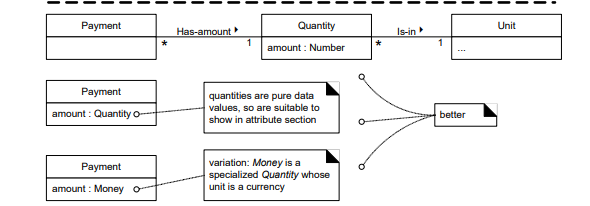
\includegraphics[width=0.3\textwidth] {Resources/Images/Einheiten.png}
			\caption{\label{fig:Einheiten}Einheiten}
	\end{figure} 
	\end{itemize}
	\item \textcolor {teal} {\textbf{Zeitintervalle}}
	\begin{itemize}
		\item Gültigkeitsintervall für sich ändernede Attribute : \begin{figure}[H]
				\centering
				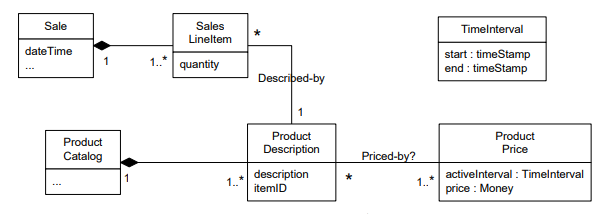
\includegraphics[width=0.3\textwidth] {Resources/Images/Zeitintervall.png}
			\caption{\label{fig:Zeitintervall}Zeitintervall}
				\end{figure} 
	\end{itemize}
\end{itemize}





















































\end{document}